\section{Three-dimensional simulations}\label{results3d}
In this section we review 3D simulations carried 
out using ZEUS-MP and PLUTO. The main purpose is to verify 
the above results with different numerical codes, and validate  
the 2D approximation.    

The 3D disc has radial size
$[r_\mathrm{min},r_\mathrm{max}]=[0.4,10]R_0$ and vertical extent  
$n_H=2$ scale-heights at $R=R_0$. The resolution is $N_r\times N_\theta\times
N_\phi=256\times32\times512$. This corresponds to about $4$ cells per
$H$ in radius. Because of the reduced resolution 
compared to 2D, we use a smooth perturbation by setting
$\delta = 10^{-3}$ and $M=1$ in Eq. \ref{randpert}. This corresponds
to a single $m=1$ disturbance in $R\in[R_1,R_2]$, which
eventually dominates in 2D simulations.  

The 3D discs are initialised in approximate equilibrium only, so we
first evolve the disc without perturbations using  
$(\lmax,\mmax)=(32,0)$ up to $t=10P_0$, during which 
meridional velocities are damped out. We then restart the simulation
with the above perturbation and $(\lmax,\mmax)=(32,32)$, and damp
merdional velocities near the radial boundaries. 

Fig. \ref{3d_ampmax} plots the amplitude of the $m=1$ spirals measured
in the ZEUS-MP and PLUTO runs.  
%why no high m
                                %modes as in 2D for iso disc?
                                %resolution? 
In the ZEUS-MP run we observe disturbances developed near
the inner boundary, which is probably responsible for the initial growth
for $t<70P_0$. This is likely a numerical artifact and effectively seeds
the ZEUS-UP simulation with a larger initial perturbation. Results
from ZEUS-MP are therefore off-set from PLUTO by $\sim50P_0$ However,
once the coherent $m=1$ spiral begins to grow ($t\gtrsim 100P_0$), 
we measure similar growth rates in both codes: 
\begin{align*}
  &\gamma \simeq 0.0073\Omega_k(R_0) \quad\quad \mathrm{PLUTO},\\
  &\gamma \simeq 0.0084\Omega_k(R_0) \quad\quad \varA{ZEUS-MP}.
\end{align*}
Both are smaller than the 2D simulations and due to the
low resolutions adopted and/or the small softening length employed in
2D.  Fig. \ref{3d_ampmax} also show results from strictly isothermal
simulations, which display no growth compared to cases with a 
temperature gradient. This confirms the temperature gradient effect is
the same in 3D. 

% We also show results from strictly
% isothermal discs ($q=0$). 
%growth rate does not depend on pert amp

\begin{figure}
  \includegraphics[width=\linewidth]{figures/m1_analysis_plot_ampmax3d.ps}
  \caption{Evolution of the maximum $m=1$ density component in  $r\in[R_1,R_2]$
    measured in the 3D simulations. Results from discs with a imposed 
    temperature gradient ($q=1$) and a strictly isothermal disc
    ($q=0$) are shown.  
    \label{3d_ampmax}}   
\end{figure}

Visualisations of the 3D simluations are shown in   
Fig. \ref{3d_prelim} for the disc midplane and near the upper disc
boundary. The snapshots are chosen when the one-armeded spirals in the two codes
have reached similar amplitudes. The agreement between the codes,
as well as with the 2D simulations, is satisfactory. Away from the
disc midplane, a coherent spiral arm is not prominent, but the
disturbance is radially more global, extending up to $R\sim 4R_0$.   
%implications?

\begin{figure}
  \begin{center}
    \subfigure[ZEUS-MP]{
      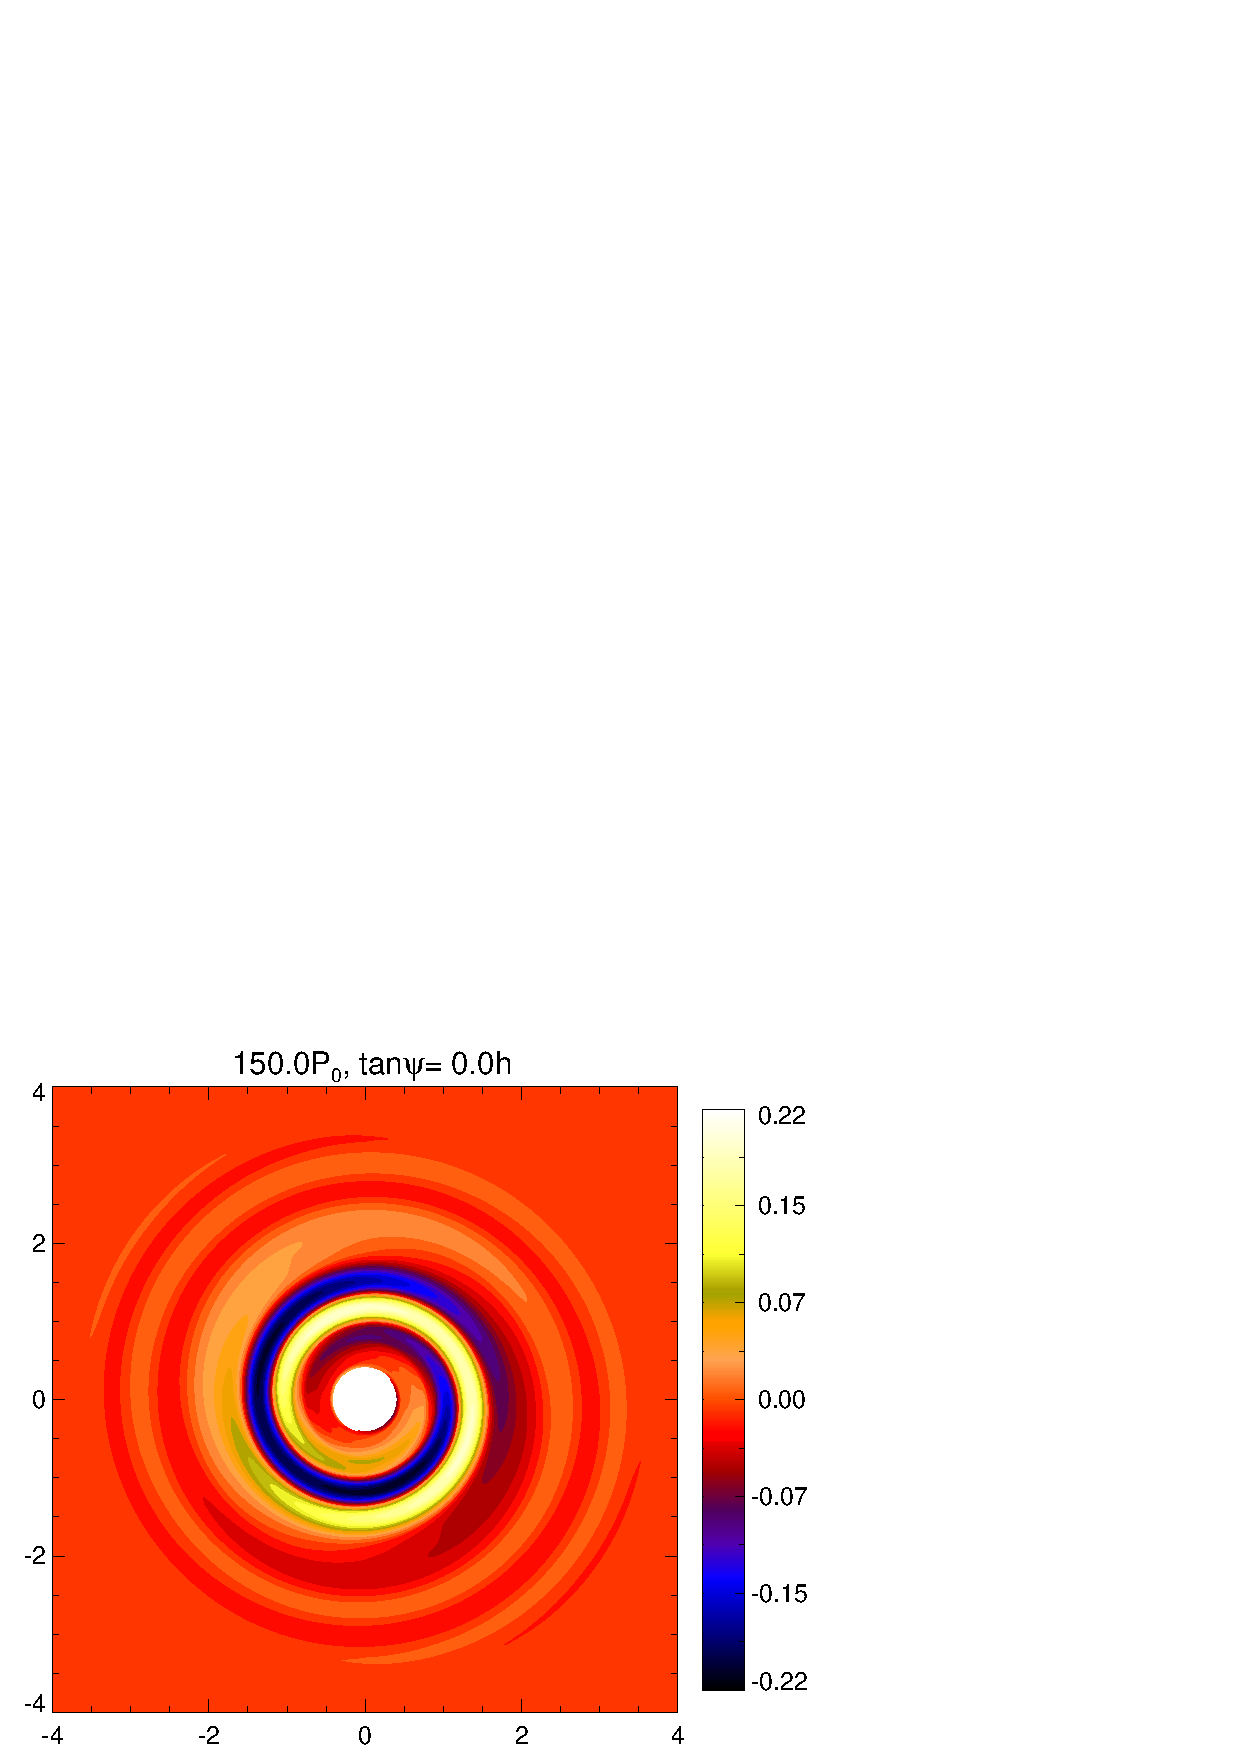
\includegraphics[scale=0.305,clip=true,trim=0cm 0cm 0cm 0cm]{figures/polarxy2_dens015_z0}  
      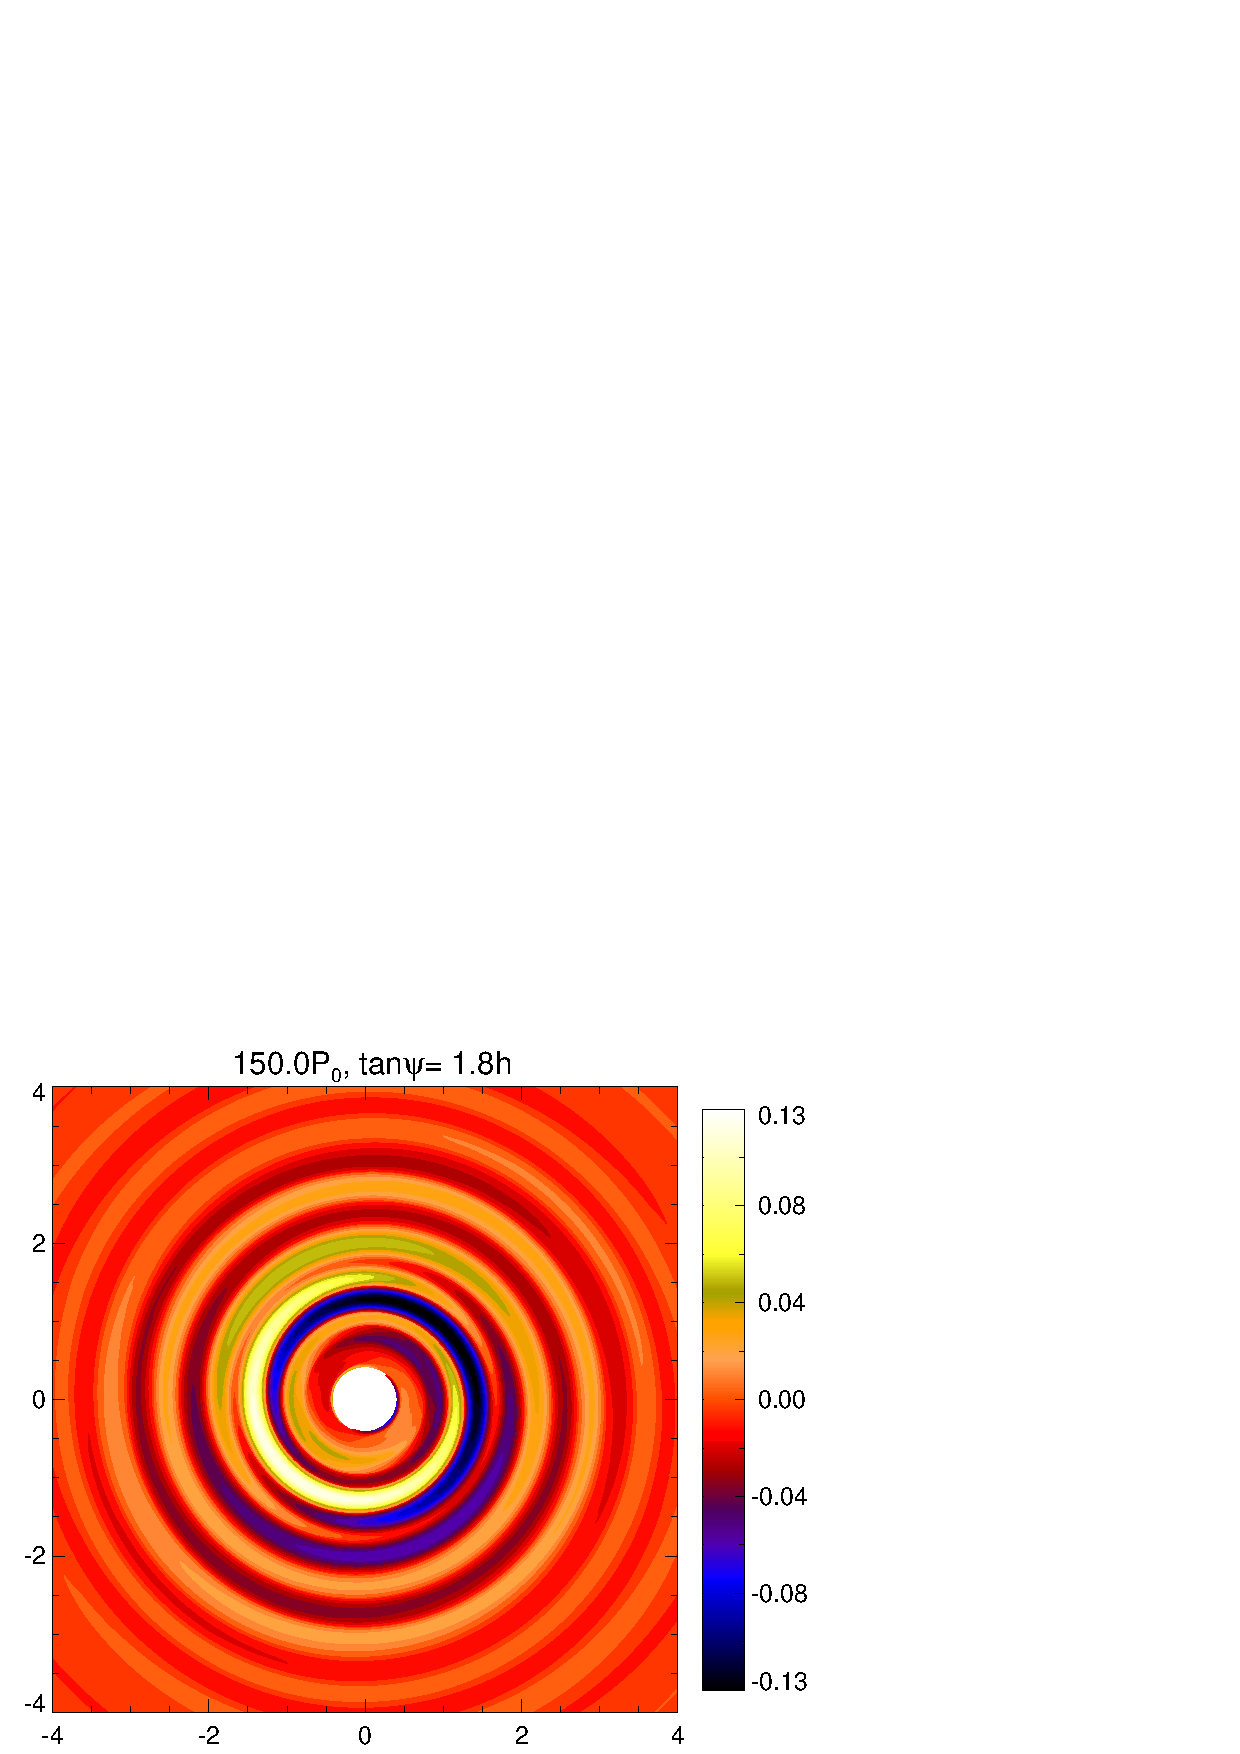
\includegraphics[scale=0.305,clip=true,trim=0.8cm 0cm 0cm
      0cm]{figures/polarxy2_dens015_zmax}  
    }
    \subfigure[PLUTO]{
      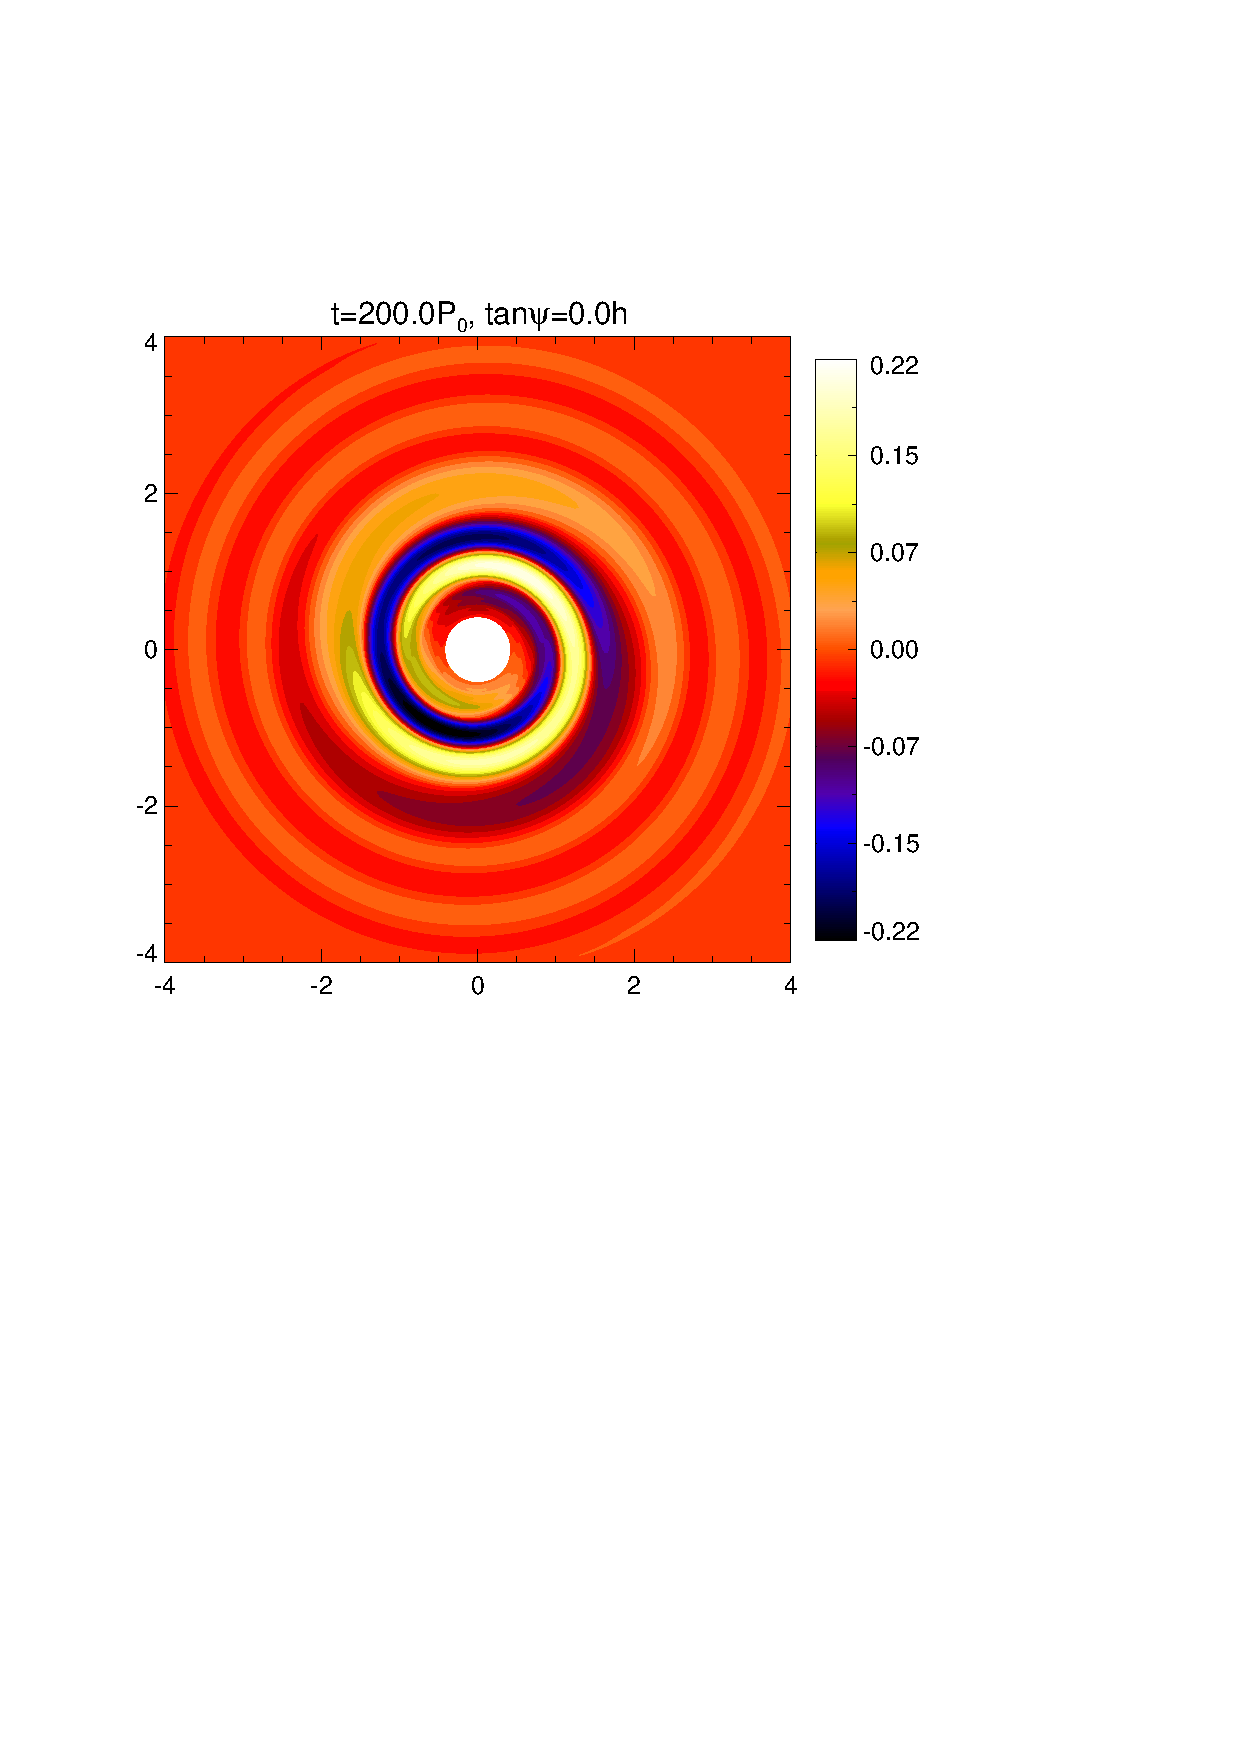
\includegraphics[scale=0.305,clip=true,trim=0cm 0cm 0cm 0cm]{figures/pdiskxy_023_z0}
      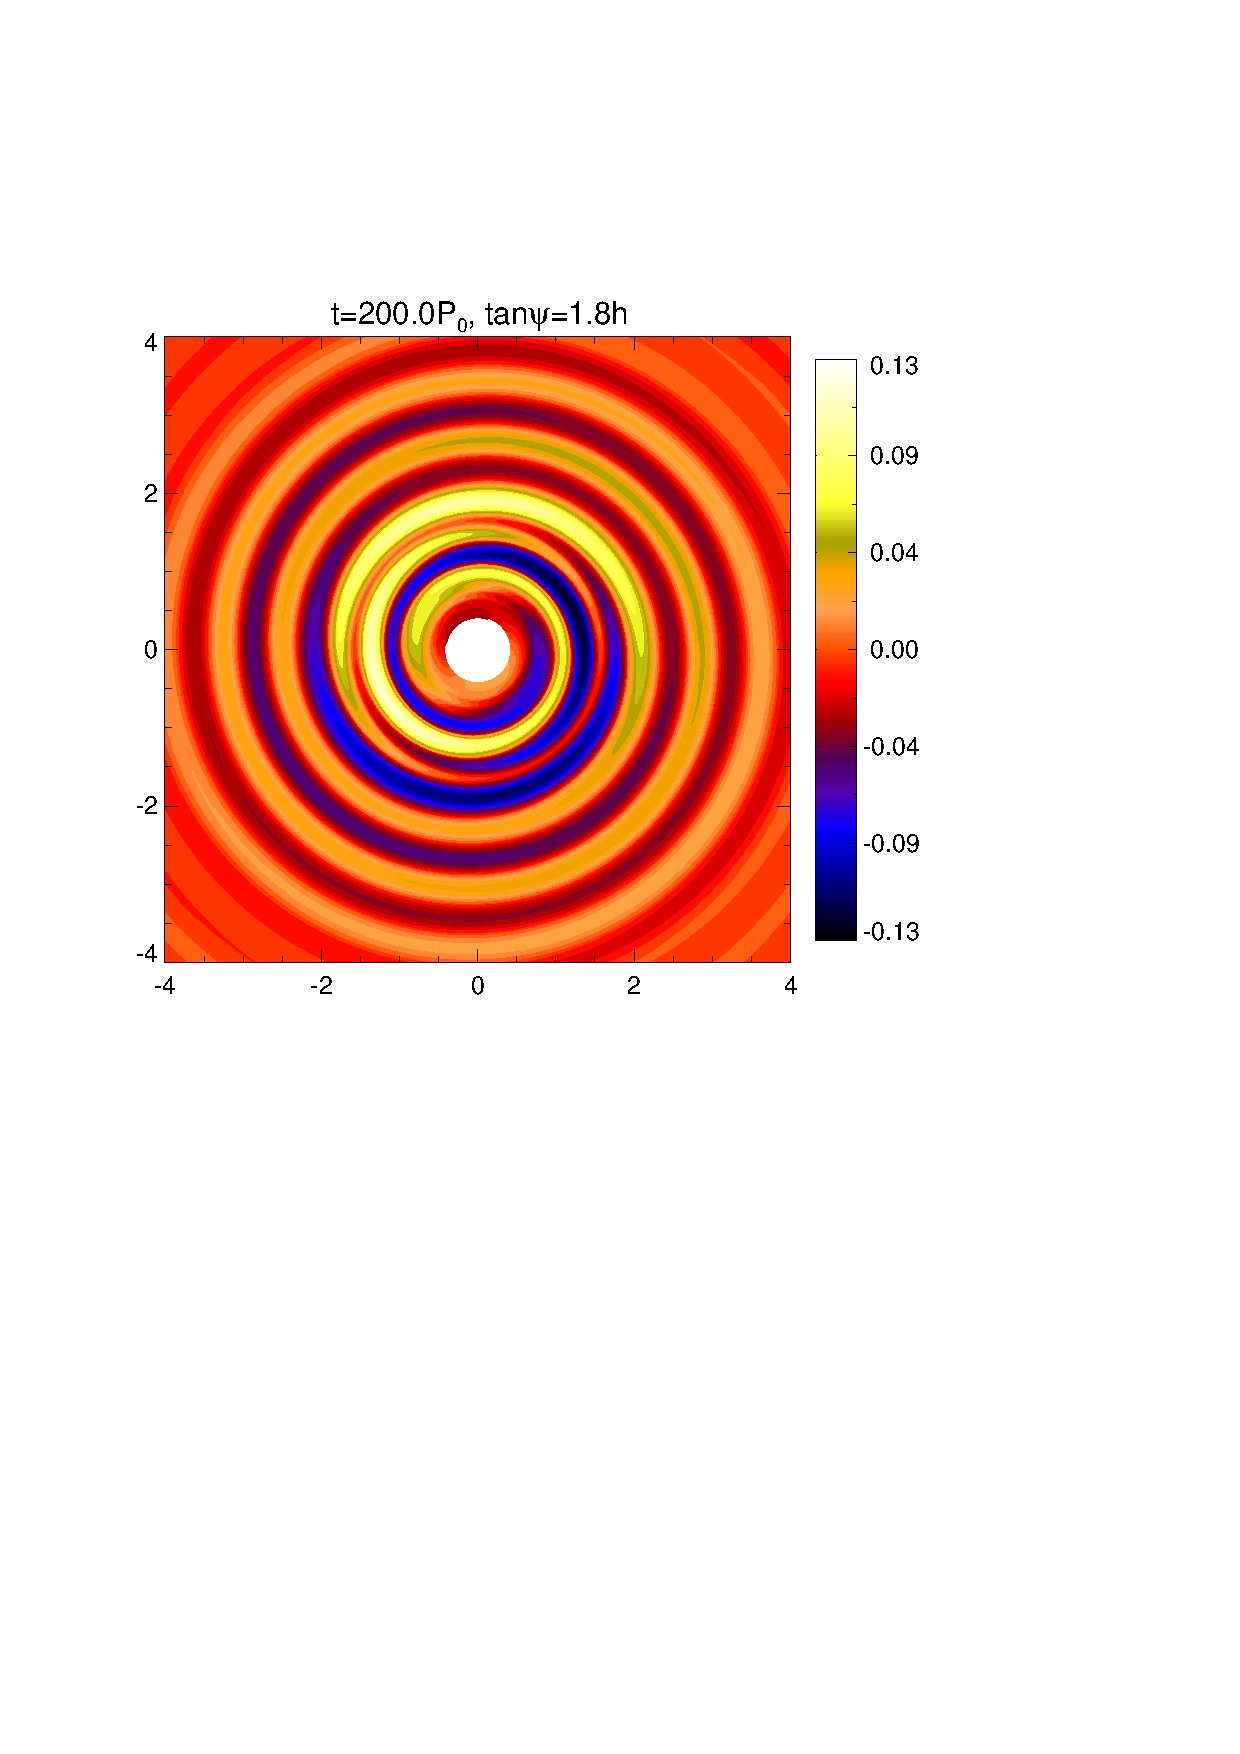
\includegraphics[scale=0.305,clip=true,trim=0.8cm 0cm 0cm
      0cm]{figures/pdiskxy_023_zmax}
    }
  \end{center}
  \caption{Three-dimensional simulations using the ZEUS-MP (top) and 
    PLUTO (bottom) codes. The $m=1$ density component $\Delta\rho_1$ at the midplane (left) and
    two scale-heights above the midplane (right) is shown. Here $\psi
    \equiv \pi/2 - \theta$ is the angular height  
    from the midplane. \label{3d_prelim}}   
\end{figure}

\subsection{Vertical structure}
Fig. \ref{3d_rz} shows the vertical structure of the one-armed
spiral in the PLUTO run. The main spiral is confined to $z < H$. Thus,
a 2D disc model, representing dynamics near the disc midplane, 
should be sufficient to study the instability. Interestingly, however, for $R>2R_0$ the
spirals  increase in amplitude away from the midplane. It remains
small in our disc model ($|\Delta\rho| < 0.1$), but could become 
significant with a larger vertical domain. The figure shows that 
the one-armed spiral can have a global influence away from the
midplane of the self-gravitating annulus.

\begin{figure}
  \includegraphics[scale=0.47,clip=true,trim=0cm 0.79cm 0cm
  0cm]{figures/pdisk_rz_023_sg.ps}  
  \includegraphics[scale=0.47,clip=true,trim=0cm 0cm 0cm
  0.64cm]{figures/pdisk_rz_023_nsg.ps}  
  \caption{Vertical distribution of the $m=1$ density component in the meridional plane from the 
    PLUTO simulation. The slices are taken at the azimuth of   
    $\mathrm{max}[\Delta\rho_1(r,\pi/2,\phi)]$. Arrows correspond to the vector 
    $(v_r/R_0,-v_\theta/rh\sin^2{\theta})$. The top (bottom) panel corresponds
    to the inner (outer) portions of the disc. 
    \label{3d_rz}} 
\end{figure}   

Although Fig. \ref{3d_rz} appears to display significant vertical motion,
the three-dimensionality parameter $\Theta < 10^{-2}$
(Eq. \ref{theta}), implying the kinetic energy associated with
vertical motion is insignificant compared to that in horizontal
motion. We find  $|v_z/c_s|\lesssim 
0.2$ for $h=0.05$. Thus, vertical motions are sub-sonic and negligible
compared to horizontal motions, which supports a 2D approximation. 

%negligible vertical motion
%unstratified approxi good?

%This again supports the 2D approximation, altthou

%Vertical velocities
%do increase with the growth of the one-armed spiral, 
%Larger amplitudes
%are reached in ZEUS because of larger numerical noise. 
%but we find  $\Theta \lesssim 10^{-2}$. 

%\begin{figure}
%  \includegraphics[width=\linewidth]{figures/m1_analysis_plot_vert.ps}
% \caption{Evolution of three-dimensionality $\Theta$, as defined by
%    Eq. \ref{theta}, which corresponds to the
%   average vertical kinetic energy density, scaled by 
%    the average horizontal kinetic energy.\label{3d_vert}} 
%\end{figure}   

\subsection{Angular momentum conservation} 
Fig. \ref{3d_angmom} shows the angular momentum evolution in the 3D
runs. ZEUS-MP does not conserve angular momentum very well, but the
variation $|\Delta J/J|< O(10^{-6})$ is small compared 
to the individual components $|\Delta J_{0,1}/J|\sim 
5\times10^{-5}$. The PLUTO run reaches similar values of
$|J_{0,1}|$, but achieves better conservation, with $|\Delta
J/J|=O(10^{-8})$. These plots are again similar to the 2D simulations,
i.e. angular momentum lost by $J_1$ is gained by $J_0$. This confirms 
that the interaction between $J_1$ and $J_0$ operates in 3D and 2D
similarly.  

\begin{figure}
%scale=0.41
  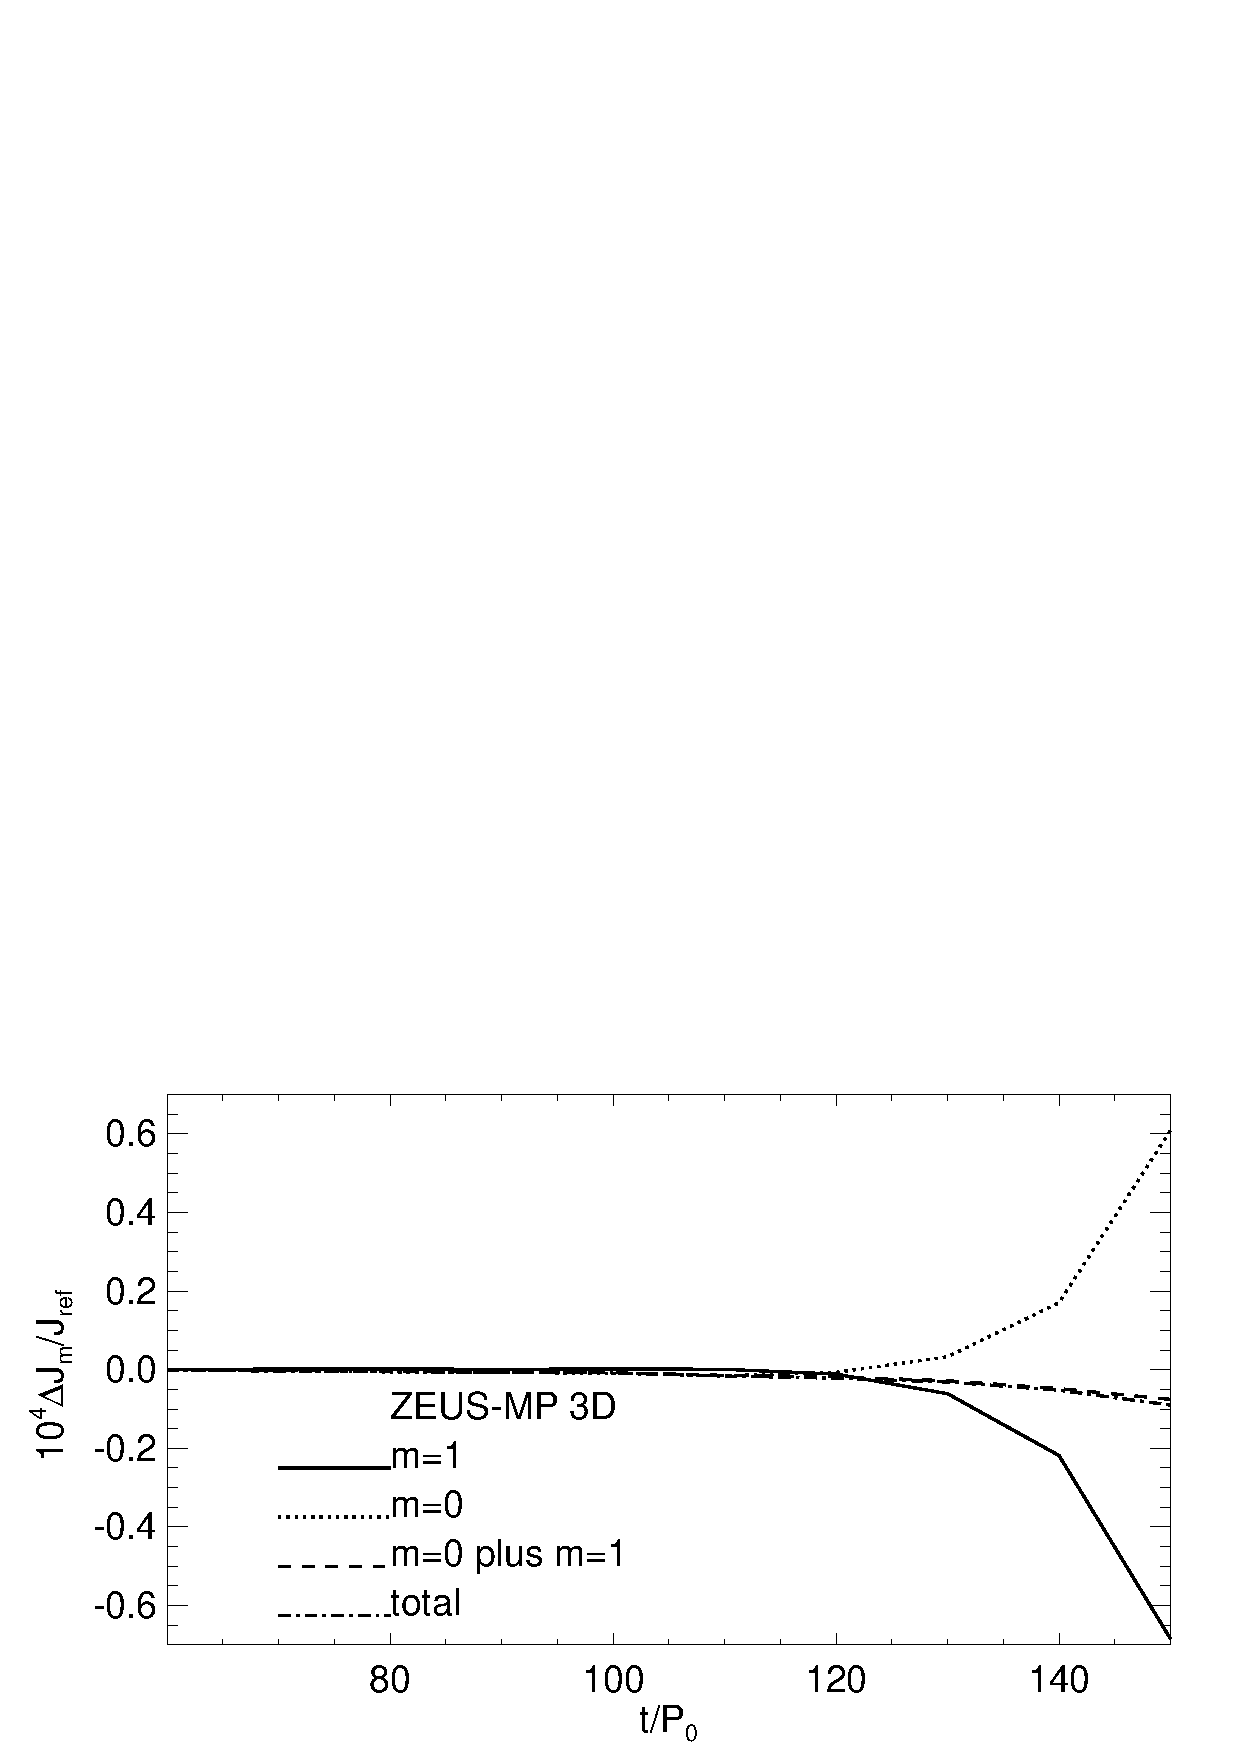
\includegraphics[scale=.41,clip=true,trim=0cm 1cm 0cm 0cm]{figures/nonaxi_evol_ang_zeus}
  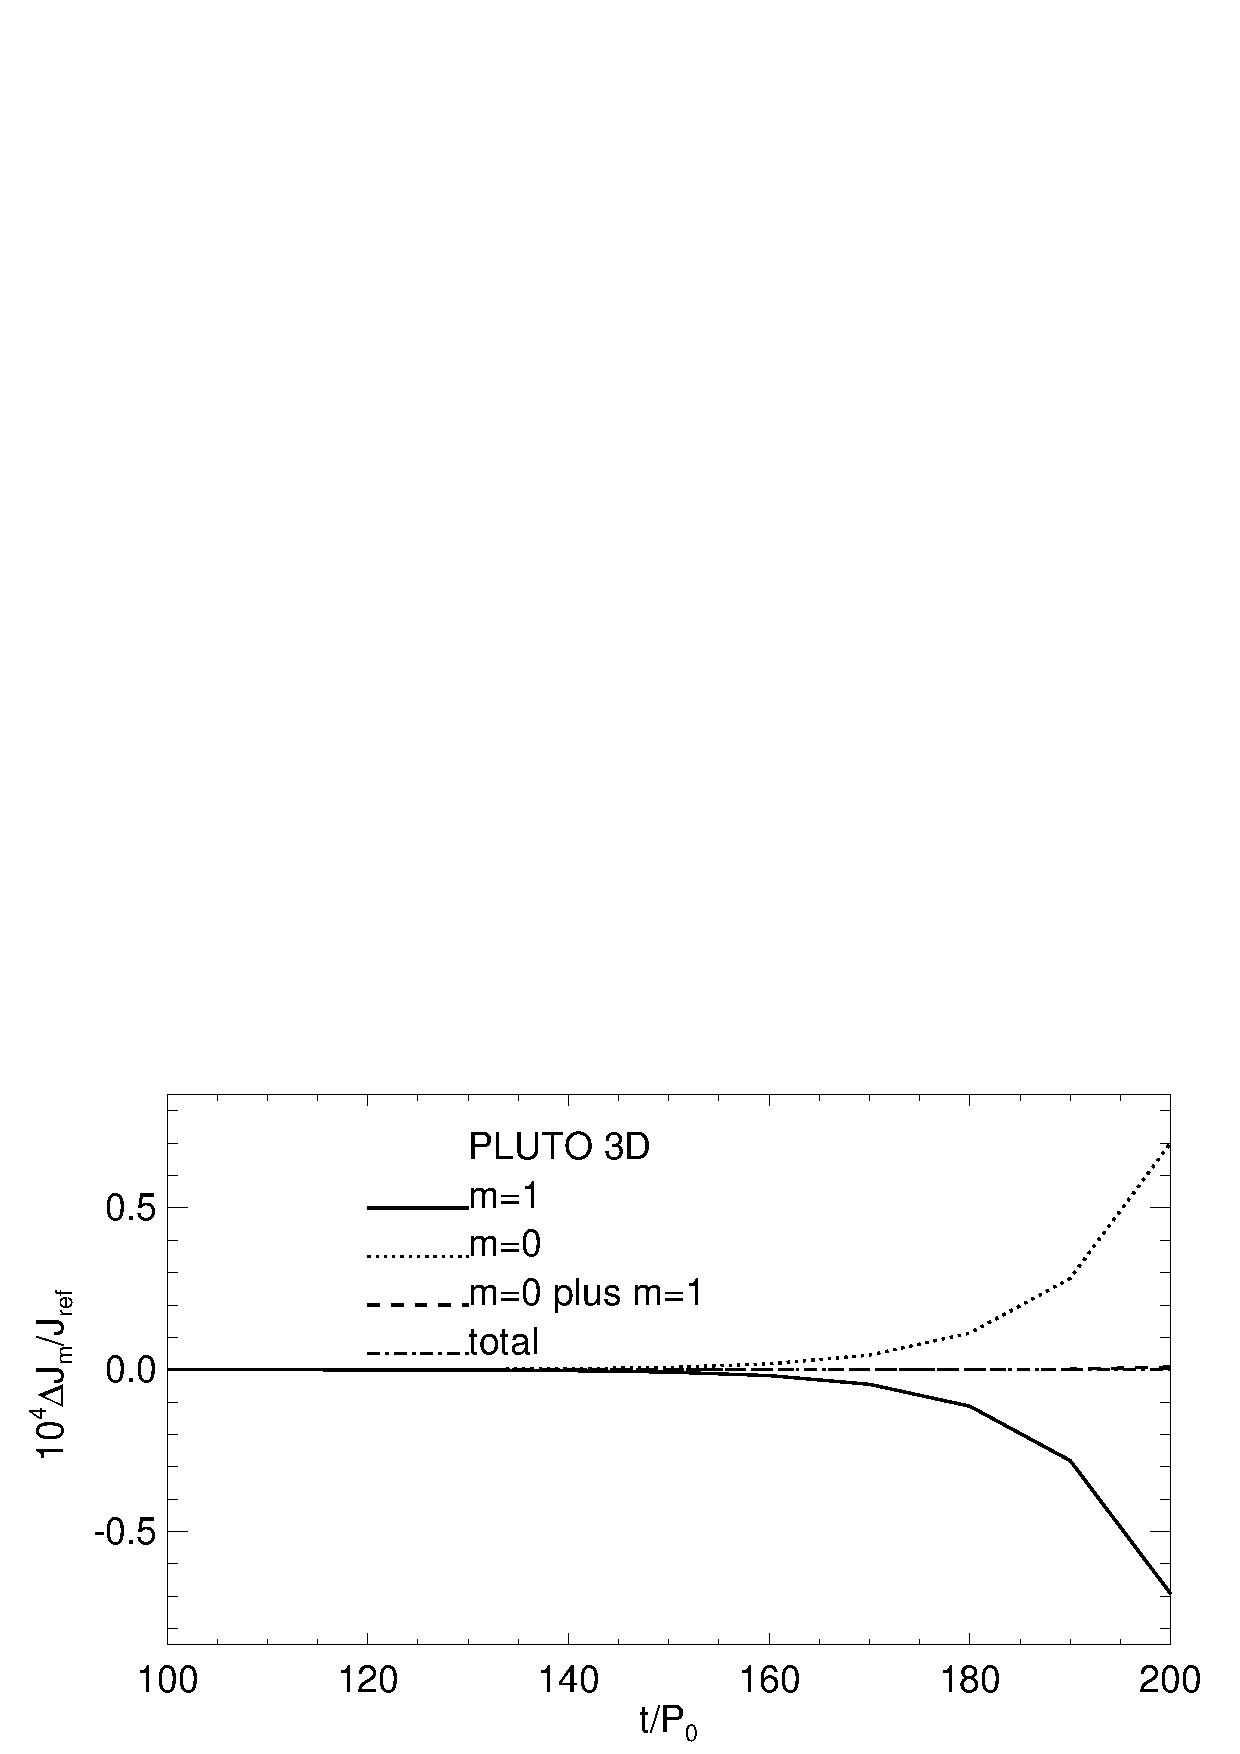
\includegraphics[scale=.41]{figures/nonaxi_evol_ang_pluto}
  \caption{Evolution of angular momentum components in the 3D 
    simulations. The perturbation 
    relative to $t=10P_0$, during the growth of the one-armed spiral,
    is shown in units of the initial total angular momentum
    $J_\mathrm{ref}$.\label{3d_angmom}}  
\end{figure}   

